%META {"question":"Đường thẳng zt chứa tia phân giác Oz của góc xOy. Đường thẳng zt được gọi là gì?","options":["Đường phân giác của góc xOy","Tia phân giác của góc xOy","Đường trung trực của đoạn thẳng","Tia đối của tia Ox"],"answer":0,"note":"Đường thẳng chứa tia phân giác của một góc gọi là đường phân giác của góc đó."}
\documentclass[border=5pt]{standalone}
\usepackage{tkz-euclide}
\usetikzlibrary{arrows.meta}
% Màu dùng chung cho toàn bộ hình vẽ (ảnh stack với nền tối của web)
\definecolor{tminc}{RGB}{226,232,240}   % chữ + nét chính
\definecolor{tmblue}{RGB}{0,210,255}    % nhấn neon xanh
\definecolor{tmpink}{RGB}{255,0,200}    % nhấn neon hồng
\definecolor{tmgreen}{RGB}{0,255,136}   % nhấn neon xanh lá
\color{tminc}

\begin{document}
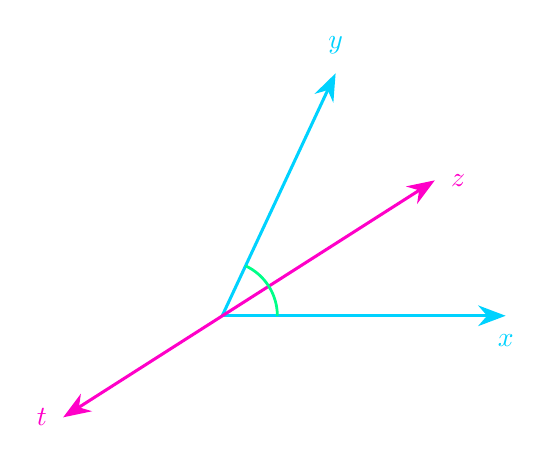
\begin{tikzpicture}[line width=1.1pt,>={Stealth[length=3.5mm]}]
  \coordinate (O) at (0,0);
  \coordinate (X) at (3.6,0);
  \coordinate (Y) at (1.44,3.08);
  \coordinate (Z) at (2.7,1.72);
  \coordinate (T) at (-2.02,-1.29);
  \draw[tmblue,->] (O) -- (X) node[below=3pt]{$x$};
  \draw[tmblue,->] (O) -- (Y) node[above=3pt]{$y$};
  \draw[tmpink,<->] (T) -- (Z) node[pos=0,left=2pt]{$t$} node[pos=1,right=2pt]{$z$};
  \tkzMarkAngles[size=0.7,arc=l,color=tmgreen,line width=1pt](X,O,Z)
  \tkzMarkAngles[size=0.7,arc=l,color=tmgreen,line width=1pt](Z,O,Y)
\end{tikzpicture}
\end{document}
